% !TeX encoding=utf8
% !TeX spellcheck = de-DE

\chapter{Applikation}

Dieses Kapitel beschreibt den Entwicklungsverlauf unserer Applikation, die zugrundeliegenden Algorithmen und Datenstrukturen, sowie das Klassenmodell und die Interaktionen zwischen den verschiedenen Applikations-Schichten.

Programmausschnitte werden  in Python-Code wiedergegeben.

\section{Algorithmus}

\paragraph*{}
Der Ameisen Optimierungs-Algorithmus ist in den Grundzügen einfach. Eine gewisse Anzahl autonomer Agenten (Ameisen) bewegt sich ausgehend von einem Nest-Knoten entlang eines Graphen bis zu einem Futter-Knoten. Die Ameise muss sich bei jedem Knoten entscheiden, über welche Kante sie zum nächsten gelangen möchte. Diese Entscheidung basiert hauptsächlich auf der Menge von Pheromonen, welche sich auf dieser Kante befinden. Dies wird wiederholt, bis die Ameise den Futterknoten erreicht. Danach befindet sie sich auf dem Rückweg zum Nest. Sie geht denselben Weg, den sie gekommen ist zurück und erhöht jeweils die Pheromonwerte auf den Kanten, die sie benutzt. Wenn sie das Nest erreicht hat, wird sie erneut auf den Weg geschickt.

\paragraph*{}
Programmiert könnte der Algorithmus etwa so aussehen:

\begin{lstlisting}
	def ant_algorithm(ants, graph):
		for ant in ants:
			next_edge = choose_next_edge(ant.node, graph)
			ant.node = next_edge.other_node(ant.node)
			if ant.has_solution:
				ant.update_phermone_trail(next_edge)	
		evaporate_pheromones(graph)
		reset_ants_with_solution(ants)
\end{lstlisting}

Wichtig sind natürlich die verschiedenen Funktionen, die in diesem kurzen Codeblock aufgerufen werden:

\begin{description}
\item[choose\_next\_edge] Bestimmt auf der Grundlage von verschiedenen Parametern, die wir jetzt noch nicht kennen, welche Kante die Ameise als nächstes besuchen wird.
\item[update\_pheromone\_trail] Erhöht die Pheromonmenge auf einer Kante des Graphen.
\item[evaporate\_pheromones] Verringert die Menge an Pheromonen auf einer Kante des Graphen.
\item[reset\_ants\_with\_solution] Die Ameisen, die mit einer fertigen Lösung wieder beim Nest angekommen sind, werden zurückgesetzt und können wiederverwendet werden. 
\end{description}

\subsection{Ablauf und Formeln}

Für die verschiedenen Teilschritte sind ein paar wenige, einfache Formeln nötig. Sie werden benötigt um die Wahrscheinlichkeit einer Kante zu ermitteln, von der Ameise ausgewählt zu werden, die Menge an Pheromonen zu bestimmen, die eine Ameise auf einer Kante hinterlässt und die bei der Evaporation verringert wird.

\paragraph*{}
Für die Betrachtung der verschiedenen Formeln soll folgender Graph als Grundlage dienen:

\paragraph*{}
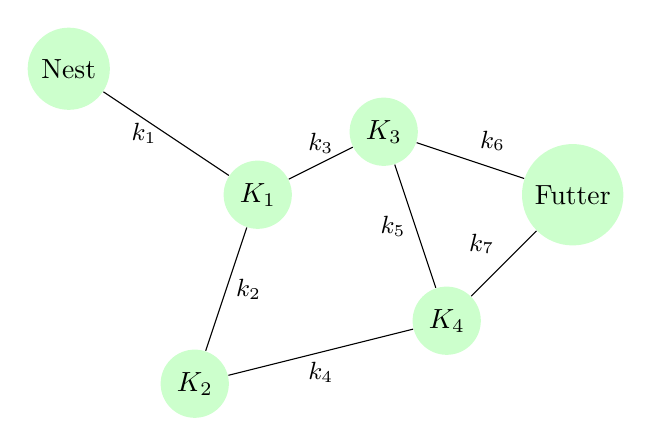
\begin{tikzpicture}
  [scale=.8,auto=left,every node/.style={circle,fill=green!20}]
  \node (nn) at (3,10) {Nest};
  \node (n1) at (6,8)  {$K_1$};
  \node (n3) at (8,9)  {$K_3$};
  \node (nf) at (11,8) {Futter};
  \node (n4) at (9,6)  {$K_4$};
  \node (n2) at (5,5)  {$K_2$};

  \path[every node/.style={font=\sffamily\small}]
    (nn) edge node [left] {$k_1$} (n1)
    (n1) edge node [right] {$k_2$} (n2)
         edge node [above] {$k_3$} (n3)
    (n2) edge node [below] {$k_4$} (n4)
    (n3) edge node [left] {$k_5$} (n4)
         edge node [above right] {$k_6$} (nf)
    (n4) edge node [above left] {$k_7$} (nf);
\end{tikzpicture}

\subsubsection*{Exploration}

Solange die Ameise keinen Futterknoten gefunden hat, befindet sie sich in der Explorationsphase (Erkundungsphase). Wir nehmen an, dass sie sich momentan beim Knoten $K_1$ befindet. Sie hat bis dahin bereits die Knoten $\{Nest\}$ besucht. Um Loops zu vermeiden, ist es einer Ameise nicht gestattet, einen Knoten zweimal zu besuchen. Die Menge der begehbaren Kanten ist demnach $\{k_3, k_2\}$. Die Pheromonwerte an den beiden Kanten sind $\{phero_{k_3}, phero_{k_4}\}$. 

Die Wahrscheinlichkeit für eine Kante berechnet sich durch:

\[ p_{k_i} = \frac{phero_{k_i}^\alpha}{\sum\nolimits_{i=0}^n phero_{k_i}^\alpha} \]

Der Exponent $\alpha$ ist eine experimentell festgestellte Grösse und wird in der Literatur mit $2$ angegeben. Um den Exponenten vernünftig anwenden zu können, müssen sich die Pheromonwerte zwischen $0$ und $1$ befinden, ansonsten ist das Resultat nicht vorhersehbar. Dies erreicht man, indem man die maximale Menge an Pheromonen auf den zur Auswahl stehenden Kanten ermittelt und folgende Formel auf alle Pheromonwerte anwendet. Als untere Grenze ($phero_{min}$) wird jeweils $0$ verwendet.

\[ phero_{k_i} = \frac{phero_{k_i} - phero_{min}}{phero_{max} - phero_{min}} \] 

Wie man gleich an einem Rechenbeispiel erkennen kann, verstärkt der Exponent $\alpha$ die Unterschiede zwischen den Pheromonwerten. 

\paragraph*{Rechenbeispiel}

Wir betrachten immer noch den Fall von oben und nehmen für die Pheromonwerte der Kanten $k_3$ und $k_4$ die Werte $phero_{k_3} = 15 $ und $phero_{k_4} = 46$ an. Zuerst müssen wir diese Werte auf Zahlen zwischen $0$ und $1$ normieren:

\begin{equation*}
\begin{split}
phero_{k_3} & = \frac{phero_{k_3} - phero_{min}}{phero_{max} - phero_{min}} \\
            & = \frac{15 - 0}{46 - 0} \\
            & = 0.37
\end{split}
\end{equation*}

\begin{equation*}
\begin{split}
phero_{k_4} & = \frac{phero_{k_4} - phero_{min}}{phero_{max} - phero_{min}} \\
            & = \frac{46 - 0}{46 - 0} \\
            & = 1
\end{split}
\end{equation*}

Ohne $\alpha$ zu beachten, wären die Zähler der Wahrscheinlichkeitsformel nun $0.37$ und $1$. Die Differenz ist demnach $1 - 0.37 = 0.63$. Wenn $\alpha = 2$ verwendet wird, betragen die Werte $0.37^2 = 0.1369$ und $1^2 = 1$. Die Differenz ist nun $1 - 0.1369 = 0.8631$. Es wird also wahrscheinlicher, dass $k_4$ als nächste Kante gewählt wird.

Die berechneten Wahrscheinlichkeiten für beide Kanten betragen mit $\alpha = 2$

\begin{equation*}
\begin{split}
p_{k_3} & = \frac{0.37^2}{0.37^2 + 1^2} \\
        & = 0.12
\end{split}
\end{equation*}

\begin{equation*}
\begin{split}
p_{k_4} & = \frac{1^2}{0.37^2 + 1^2} \\
        & = 0.88
\end{split}
\end{equation*}

Die Kante $k_4$ hat demnach eine ca. 7 mal höhere Chance, als nächste ausgewählt zu werden als $k_3$

Um die nächste Kante tatsächlich auswählen zu können, werden die Wahrscheinlichkeiten gewichtet und durch eine Zufallszahl ausgewählt. Dazu wird zuerst ein n-Tupel der Form $(p_0, p_0 + p_1, p_0 + p_1 + p_2, ..., \sum\nolimits_{i=0}^n p_n)$ erstellt. Danach generiert man eine Zufallszahl zwischen $0$ und $1$ und ermittelt mittels Bisektion den korrespondierenden Wert im Tupel. Unser Tupel besteht nur aus zwei Einträgen $(0.12, 0.12 + 0.82) = (0.12, 1)$. $k_3$ wird ausgewählt, wenn sich die Zufallszahl zwischen $0$ und $0.12$, $k_4$, wenn sie sich zwischen $0.12$ und $1.0$ befindet. 

\paragraph*{Erweiterung}

Die oben aufgeführte Formel zur Berechnung der Wahrscheinlichkeit lässt sich auf einfache Weise durch einen bekannten Wert erweitern und beinflussen. In unserem Fall sind das die Kosten der jeweiligen Kante $cost_{k_i}$. Die Kosten sollen die Wahrscheinlichkeit gegebenenfalls nach unten korrigieren. Die angepasste Formel lautet

\[ p_{k_i} = \frac{phero_{k_i}^\alpha \cdot cost_{k_i}^\beta}{\sum\nolimits_{i=0}^n phero_{k_i}^\alpha \cdot cost_{k_i}^\beta} \] 

Auch hier müssen die Kosten normiert werden. Das Ziel ist, die Wahrscheinlichkeit stärker mehr zu verringern, je grösser die Kosten der entsprechenden Kante sind. Das heisst, dass wenn der Kostenwert zwischen $0$ und $1$ normiert wird, höhere Kosten näher bei $0$ und tiefere näher bei $1$ sein müssen. Dies wird durch die folgende Normierungsformel erreicht:

\[ cost_{k_i} = \frac{1}{\frac{cost_{k_i}}{cost_{min}}} \]

In unserem Beispiel sind die neuen Kosten demnach

\begin{equation*}
\begin{split}
cost_{k_3} & = \frac{1}{\frac{15}{15}} \\
           & = 1
\end{split}
\end{equation*}

\begin{equation*}
\begin{split}
cost_{k_4} & = \frac{1}{\frac{46}{15}} \\
           & = \frac{15}{46}
           & = 0.33
\end{split}
\end{equation*}

Das bedeutet, dass bei der Auswertung der Wahrscheinlichkeit von $k_4$ die Pheromonwerte mit $0.33$ multipliziert und dadurch verringert werden. Die Unterschiede zwischen den Kosten-Modifikatoren kann durch $\beta$ beeinflusst werden. Hohe Werte verstärken die Unterschiede, Werte zwischen $0$ und $1$ verringern sie.

\subsubsection*{Exploitation (Verwertung)}

Die zweite Phase des Algorithmus ist die Verwertung des Ergebnissen. Sie beginnt, wenn die Ameise den Futterknoten erreicht. In dem Moment geht sie den von ihr gefundenen Pfad zurück und erhöht die Pheromonmenge auf jeder Kante, die sie entlang läuft.

Die Menge an Pheromonen hängt dabei direkt von der gefundenen Pfadlänge ab:

\[ phero_{inc} = {\frac{1}{pathlength}}^\gamma \]

Der neue Pheromonwert beträgt danach 

\[ phero_{k_i} = phero_{k_i} + phero_{inc} \]

Das heisst, dass bei längeren Pfaden generell weniger Pheromone platziert werden. Der Exponent $\gamma$ verstärkt die Unterschiede zwischen den Mengen, genau wie das $\alpha$ und $\beta$ in der Formel zur Berechnung der Wahrscheinlichkeiten. Die Pfadlänge muss immer $> 1$ sein. Dies kann bei der Erstellung des Graphen sichergestellt werden.

Sobald die Ameise das Nest erreicht, verliert sie die aktuelle Lösung und beginnt wieder von vorn.

\paragraph*{Erweiterung}

Eine sinnvolle, auch von uns implementierte Erweiterung ist die Reduzierung der addierten Menge an Pheromonen, falls sich bereits eine grosse Menge auf der Kante befindet. Dies verhindert, dass auf einer Kante immer mehr Pheromone abgelagert werden, was dazu führen würde, dass andere Kanten keine Chance mehr hätten, ausgewählt zu werden.

Dazu errechnen wir einen Multiplikator. Der Multiplikator soll nah an $0$ sein, wenn die sich bereits auf der Kante befindende Menge an Pheromonen gross ist und nah an $1$, wenn dieser Wert klein ist.

Dazu speichern wir zu jeder Zeit die maximale Anzahl Pheromone, die sich auf einer Kante im Graph befinden in $phero_{max}$ (das Maximum über alle Kanten des Graphen gesehen). Die Menge auf einer spezifischen Kante ist $phero_{k_i}$. Daraus errechnet sich folgender Multiplikator:

\[ phero_{mul} ={ 1 - \frac{phero_{cur}}{phero_{max}}}^\delta \]

Dies führt zu folgender Formel zur Berechnung der Menge an Pheromonen, die zur bestehenden hinzu addiert werden soll:

\[ phero_{inc} = phero_{inc} * phero_{mul} \]

$\delta$ ist wie bereits mehrmals erwähnt zur Gewichtung und beträgt in unserer Implementation standardmässig 0.1.

Rechenbeispiel: Die maximale Menge an Pheromonen im Graph sei $phero_{max} = 13$, die Mengen auf den Knoten $k_1 = 5$ und $k_2 = 12$. Das ergibt für $phero_{mul_{k_1}} = 1 - \frac{5}{13} = 0.62$ und $phero_{mul_{k_2}} = 1 - \frac{12}{13} = 0.08$. Man sieht, dass auf die Kante mit höherer Konzentration viel weniger dazu addiert wird als auf die mit der geringeren Konzentration. 

\subsubsection*{Evaporation}

Im letzten Schritt werden die Pheromonwerte auf allen Kanten verringert. Die Verringerung ist kein absoluter Wert, ansonsten würden früher oder später Zahlen $< 1$ erreicht. Daher errechnet sich der neue Pheromonwert einer Kante bei einer Reduktion von $\epsilon \in [0, 1]$ durch

\[ phero_{k_i} = (1 - \epsilon) \cdot phero_{k_i} \]

Das ergibt z.B. bei einer Pheromonmenge $phero_{k_i} = 10$ und $\epsilon = 0.01$ einen neuen Wert von $phero_{k_i} = 0.99 * 10 = 9.9$. $0.01$ ist zugleich der in der Literatur empfohlene Standardwert für die Reduktion.

\section{Aufbau der Applikation}

Die Applikation besteht hauptsächlich aus zwei unterschiedlichen voneinander losgelösten Teilen: dem Benutzerinterface (GUI) und der Simulation (Backend).

Die Simulation kennt dabei die GUI-Schicht nicht, sondern wird von ihr angesprochen, wenn weitere Schritte des Algorithmus berechnet werden sollen.

\subsection{Klassendiagramm}



\section{Vorgehen bei der Programmierung}

Wie unseren Release-Zusammenfassungen zu entnehmen ist, haben wir uns am Anfang primär auf die Entwicklung einer lauffähigen Version mit graphischer Darstellung konzentriert, in der sich Ameisen nach gewissen Regeln fortbewegen. 

\section{Mockups}

Zwei verschiedene Varianten für das spätere Aussehen des Programms standen im Vordergrund: eine mit der Einstellungsleiste im oberen Fensterbereich, eine zweite mit den Einstellungen am rechten Seitenrand.

\begin{figure}[h]
  \centering
	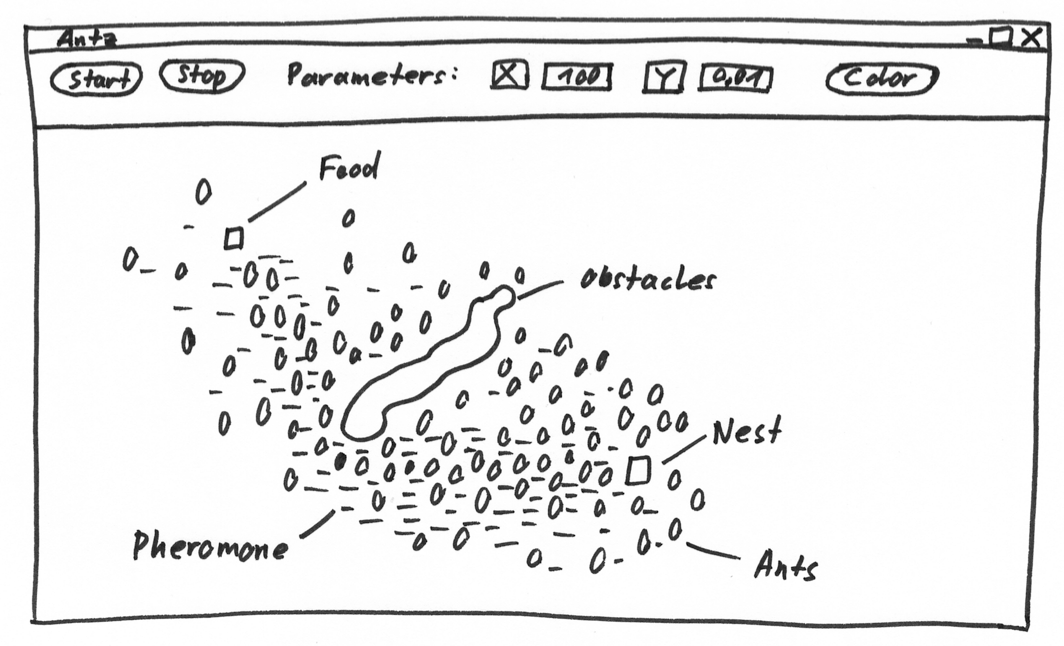
\includegraphics [width=0.85\textwidth]{images/Antz_Mockup_1_sw.png} 
	\caption{Mockup-Variante 1: Einstellungen im oberen Fensterbereich}
\end{figure}

\begin{figure}[h]
  \centering
	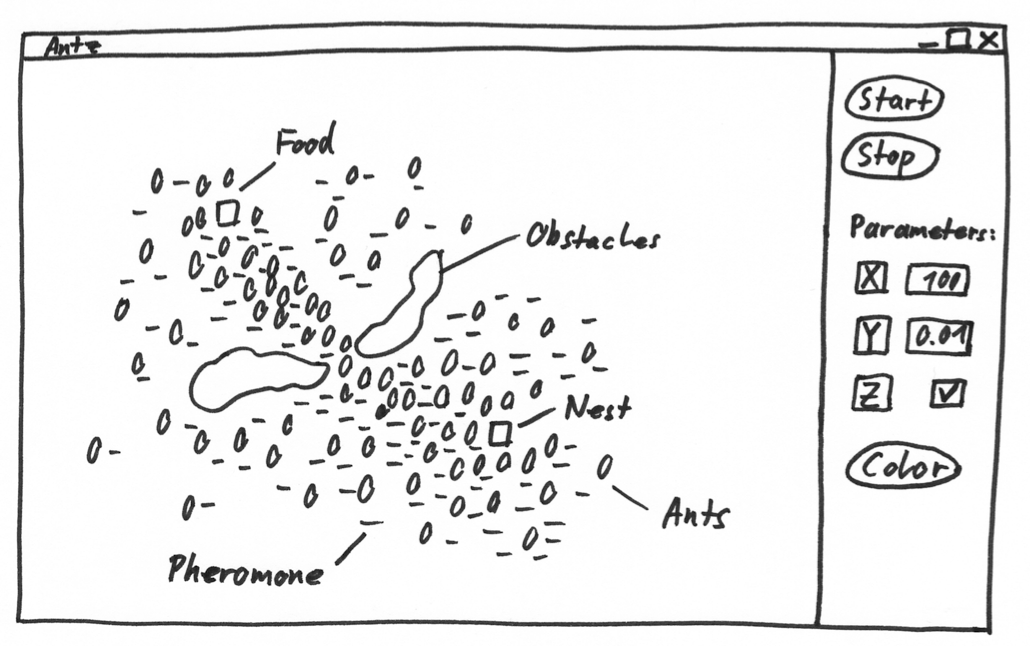
\includegraphics [width=0.85\textwidth]{images/Antz_Mockup_2_sw.png} 
	\caption{Mockup-Variante 2: Einstellungen im rechten Fensterbereich}
\end{figure}

\section{Auswertungen: Konvergenz, Parameter}

\section{Vergleich mit Dijkstra und A*}

Wir selbst haben zwar keinen Vergleich mit Dijkstra oder A* aufgestellt, trotzdem möchten wir kurz darauf eingeben und dafür die Resultate von \citet*{leo-perf} eingehen.

\citeauthor*{leo-perf} untersucht die drei Algorithmen Dijstra, A* und Ant auf ihre Effizienz beim Finden eines kürzesten Pfades. Dabei gelangt er zu folgenden Resultaten:

\begin{table}[h]
\begin{tabular}{ | l | r | }
\hline
Dijstra & ~140ms \\
\hline
A* & ~110ms \\
\hline
Ant & ~13900ms \\
\hline
\end{tabular}
\caption{Vergleich zwischen Dijkstra, A* und Ant}
\end{table}

Man kann klar erkennen, dass der Ameisen Optimierungs-Algorithmus für die Pfadfindung nicht besonders gut geeignet ist. Zu der höheren Ausführungszeit kommt noch, dass Dijstra und A* immer den optimalen Weg finden, der Ant-Algorithmus jedoch nicht zwingend.

\citeauthor*{leo-perf} untersucht auch die Eignung des Ant-Algorithmus für das Travelling Salesman Problem und gelangt dabei zu ähnlichen Ergebnissen.

\section{Screenshots}

\subsubsection*{Iteration 1}

Noch nicht implementiert, dass die Wegfindung abhängig von der Anzahl Ameisen, die durchlaufen, ist. \\

Evtl. noch eine Multi-Threaded-Lösung integrieren (sehr gut zu parallelisieren) \\

Ausserdem: schnellere Python-Interpreter wie pypy (oder für numerische Berechnungen); für z.B . 10'000 Nodes! \\

Idee: vielleicht noch Rauschen integrieren? Random von 20\,\% konvergiert überhaupt nicht mehr.

\vspace*{3cm}


Inputs von Syrus: \\

\begin{itemize}
\item Interessant wäre, das Maximum der Verlangsamung bei mehr Ameisen zu messen
\item Eventuell in Richtung Programming Tuning gehen? (Performance-Messungen: wie viel fällt auf welchen Bereich?) 
\item Für die Iterationen 2 und 3: Einsatz der Ressourcen planen (Andere Algorithmen; Optimierung; Vergleich mit Djikstra: Statistiken; vgl. Optimierungspotential bezüglich Zeit und Speicheraufwand, etc.); z.B. eher TSP (weil visuell für die Mitstudierenden ansprechender?) 
\end{itemize}